\documentclass[10pt,twocolumn]{article}

\usepackage[margin=0.58in,top=0.58in,bottom=0.62in]{geometry}
\setlength{\columnsep}{0.20in}
\usepackage{amsmath,amssymb,amsfonts,amsthm}
\usepackage{graphicx}
\usepackage{booktabs}
\usepackage{array}
\usepackage{titlesec}
\usepackage{caption}
\usepackage{enumitem}
\usepackage{xcolor}
\usepackage[colorlinks=true,linkcolor=blue!60!black,citecolor=blue!60!black,urlcolor=blue!60!black]{hyperref}

% Compact IEEE/SIAM-inspired section and float spacing
\titlespacing*{\section}{0pt}{5.5pt plus 1.5pt minus 1pt}{2.5pt plus 1pt}
\titlespacing*{\subsection}{0pt}{4pt plus 1pt minus 1pt}{1.5pt}
\titleformat{\section}{\normalfont\fontsize{10.5}{12}\bfseries}{\Roman{section}.}{0.5em}{}
\titleformat{\subsection}{\normalfont\fontsize{9.5}{11}\bfseries\itshape}{\Alph{subsection}.}{0.4em}{}
\captionsetup{font={footnotesize},labelfont={bf},skip=3pt}
\setlength{\textfloatsep}{7pt plus 2pt minus 2pt}
\setlength{\floatsep}{6pt plus 2pt minus 2pt}
\setlength{\intextsep}{6pt plus 2pt minus 2pt}
\setlength{\abovedisplayskip}{4.5pt plus 1pt minus 1pt}
\setlength{\belowdisplayskip}{4.5pt plus 1pt minus 1pt}
\setlist[itemize]{nosep,leftmargin=1.2em,topsep=2pt}

\newtheorem{proposition}{Proposition}

\title{\vspace{-1.0em}\textbf{\Large Development and Evaluation of Algorithmic Trading Strategies Using Mean-Reverting Stochastic Processes: Ornstein--Uhlenbeck and Cox--Ingersoll--Ross Models}\vspace{-0.4em}}

\author{
\normalsize MAC F244: Stochastic Calculus and Application to Finance (Semester I, AY 2026--2027)\\
\footnotesize Group Members: Kavin Kashyap Albal (\texttt{2024ADPS0832G}), Sanjan Ganesan (\texttt{2024ADPS0833G}),\\
\footnotesize Atharva Sandeep Agarwala (\texttt{2024ADPS0856G}), Shaurya Manjkhola (\texttt{2024ADPS0880G}) --- Department of Mathematics, BITS Pilani
\vspace{-0.8em}
}
\date{}

\begin{document}
\maketitle

\begin{abstract}
\noindent Financial state variables governed by restorative economic equilibrium---such as cointegrated dual-class equity spreads and sovereign bond yields---violate the unbounded variance assumption of Geometric Brownian Motion. We formulate, calibrate, and empirically backtest continuous-time algorithmic trading strategies driven by two canonical mean-reverting Stochastic Differential Equations (SDEs): the Ornstein--Uhlenbeck (OU) Gaussian diffusion and the Cox--Ingersoll--Ross (CIR) square-root diffusion. We structure the project into two decoupled, independent pillars: (i) an equity statistical arbitrage pairs strategy on Alphabet dual-class shares (\texttt{GOOGL}/\texttt{GOOG}) calibrated via discrete AR(1) Ordinary Least Squares (OLS) / Gaussian Maximum Likelihood Estimation (MLE); and (ii) a fixed-income duration regime strategy on 10-Year US Treasury yields (\texttt{\^{}TNX}) calibrated via Euler-discretized Weighted Least Squares (WLS). Across a 6-year daily dataset ($N=1{,}510$, 2019--2024) split into an in-sample calibration window (2019--2022, $\approx 70\%$) and an out-of-sample backtest window (2023--2024, $\approx 30\%$), our market-neutral OU pairs strategy delivers a $+2.49\%$ net return, a $0.83$ Sharpe ratio, a $94.4\%$ win rate, and an extraordinary maximum drawdown of only $-1.36\%$ (slashing market risk relative to the passive Buy-and-Hold benchmark drawdown of $-22.14\%$). Simultaneously, our CIR fixed-income strategy enhances risk-adjusted returns over passive bond holding (\texttt{IEF}), boosting Sharpe from $0.17$ to $0.25$ and reducing drawdown from $-10.16\%$ to $-9.01\%$ by tactically rotating into short-term cash/bonds during yield surges.
\end{abstract}

\section{Introduction \& Economic Motivation}
Classical derivatives pricing models asset prices via Geometric Brownian Motion (GBM), $dS_t = \mu S_t\,dt + \sigma S_t\,dW_t$, under which log-prices diffuse as non-stationary martingales with variance growing linearly and without bound, $\mathrm{Var}(\ln S_t) = \sigma^2 t$. While plausible for broad equity indices over multi-decade horizons, this property contradicts state variables tethered by restorative economic forces:
\begin{itemize}
\item \textbf{Dual-Class Equity Pairs:} Shares of the same underlying corporate entity (e.g., Alphabet Class A \texttt{GOOGL} with voting rights vs.\ Class C \texttt{GOOG} without voting rights) represent identical claims on earnings, dividends, and liquidation proceeds. Idiosyncratic demand imbalances cause the price ratio to fluctuate, but economic substitution forces it to revert to equilibrium.
\item \textbf{Sovereign Interest Rates:} Nominal yields reflect central-bank monetary targets and macroeconomic equilibria. When yields surge, economic tightening dampens activity and pulls yields back down; when yields drop too low, rate bounds and inflation pressures push them back up.
\end{itemize}

Continuous-time mean-reverting modeling originated with the Ornstein--Uhlenbeck (OU) process \cite{uhlenbeck1930}, adapted to interest rates by Vasicek \cite{vasicek1977} and to pairs trading by Gatev et al.\ \cite{gatev2006} and Leung \& Li \cite{leung2015}. However, because OU innovations are state-independent and Gaussian, $X_t$ admits negative values with positive probability---appropriate for real-valued spreads, but fundamentally flawed for nominal interest rates. Cox, Ingersoll \& Ross (CIR) \cite{cir1985} resolved this defect by introducing state-dependent diffusion $\xi\sqrt{r_t}\,dW_t$, ensuring strict non-negativity when the \emph{Feller condition} ($2\kappa\theta \ge \xi^2$) is satisfied.

This study implements both models across two independent, self-contained empirical applications:
\begin{enumerate}
\item \textbf{Pillar 1 (Equities):} OU Pairs Trading on \texttt{GOOGL}/\texttt{GOOG} benchmarked against passive \textbf{Buy-and-Hold \texttt{GOOGL}}.
\item \textbf{Pillar 2 (Fixed Income):} CIR Dynamic Regime Strategy on 10Y Yields / \texttt{IEF} benchmarked against passive \textbf{Buy-and-Hold \texttt{IEF}}.
\end{enumerate}
All models are evaluated on identical 2019--2024 data under a strict $70/30$ chronological train/test split.

\section{Mathematical Formulation \& Discretization}

\subsection{Ornstein--Uhlenbeck (OU) Process}
Let $(\Omega,\mathcal{F},\{\mathcal{F}_t\}_{t\ge 0},\mathbb{P})$ carry a standard 1D Brownian motion $W_t$. The OU SDE for a real-valued cointegrated spread $X_t \in \mathbb{R}$ is
\begin{equation}
dX_t = \theta(\mu - X_t)\,dt + \sigma\,dW_t, \qquad \theta > 0,\; \mu \in \mathbb{R},\; \sigma > 0,
\label{eq:ou_sde}
\end{equation}
where $\theta$ is the annualized mean-reversion speed, $\mu$ is the long-term equilibrium mean, and $\sigma$ is the diffusion volatility. 

Applying It\^o's Lemma to the integrating factor $Y_t = f(t, X_t) = e^{\theta t}(X_t - \mu)$, with $\partial_t f = \theta e^{\theta t}(X_t-\mu)$, $\partial_x f = e^{\theta t}$, and $\partial_{xx} f = 0$, gives:
\begin{equation}
dY_t = \theta e^{\theta t}(X_t-\mu)\,dt + e^{\theta t}dX_t = \sigma e^{\theta t}\,dW_t.
\end{equation}
Integrating from $t$ to $t+\Delta t$ yields the exact strong solution:
\begin{equation}
X_{t+\Delta t} = \mu + (X_t - \mu)e^{-\theta \Delta t} + \sigma \int_t^{t+\Delta t} e^{-\theta(t+\Delta t - s)}\,dW_s.
\label{eq:ou_sol}
\end{equation}
By It\^o's Isometry, the stochastic integral is normally distributed with mean zero and conditional variance:
\begin{equation}
\mathrm{Var}\!\left(\sigma \int_t^{t+\Delta t} e^{-\theta(t+\Delta t - s)}\,dW_s\right) = \frac{\sigma^2}{2\theta}\left(1 - e^{-2\theta\Delta t}\right).
\end{equation}
Hence, the exact continuous transition law is conditionally Gaussian:
\begin{equation}
X_{t+\Delta t} \mid X_t \sim \mathcal{N}\!\left(\mu + (X_t - \mu)e^{-\theta\Delta t},\; \frac{\sigma^2}{2\theta}\!\left(1 - e^{-2\theta\Delta t}\right)\right).
\label{eq:ou_trans}
\end{equation}
As $\Delta t \to \infty$, $X_t$ converges to its stationary distribution $\mathcal{N}(\mu, \sigma_{\mathrm{eq}}^2)$ with equilibrium standard deviation $\sigma_{\mathrm{eq}} = \sigma/\sqrt{2\theta}$ and half-life $t_{1/2} = \ln(2)/\theta$.

\textbf{Discretization Bias:} Standard Euler--Maruyama discretization, $X_{n+1} = X_n + \theta(\mu - X_n)\Delta t + \sigma\sqrt{\Delta t}Z_n$, attains strong order $O(\Delta t^{1.0})$ because the diffusion coefficient $\sigma$ is constant. However, equating stationary variance reveals an upward bias $V_{\mathrm{EM}} = \frac{\sigma^2}{2\theta - \theta^2\Delta t} > \sigma_{\mathrm{eq}}^2$, diverging when $\theta\Delta t \ge 2$. Exact simulation via (\ref{eq:ou_trans}) eliminates discretization bias entirely.

\subsection{Cox--Ingersoll--Ross (CIR) Process}
For strictly positive financial state variables such as nominal yields $r_t \in \mathbb{R}_+$, the CIR SDE is
\begin{equation}
dr_t = \kappa(\theta - r_t)\,dt + \xi\sqrt{r_t}\,dW_t, \qquad \kappa, \theta, \xi > 0,\; r_0 > 0,
\label{eq:cir_sde}
\end{equation}
where $\kappa$ is the adjustment speed, $\theta$ is the long-term mean yield, and $\xi$ is the volatility parameter. The state-dependent diffusion $\xi\sqrt{r_t}$ collapses to zero as $r_t \to 0$, creating endogenous heteroskedasticity.

\begin{proposition}[Feller Positivity Criterion]
The boundary at zero is non-attainable ($\mathbb{P}(r_t > 0 \; \forall t \ge 0) = 1$) if and only if
\begin{equation}
2\kappa\theta \ge \xi^2.
\label{eq:feller}
\end{equation}
If $2\kappa\theta < \xi^2$, the origin is regular and instantaneously reflecting.
\end{proposition}
\noindent\textit{Proof Sketch:} Feller's scale function $s(x) = \int^x \exp\!\left(-2\int^y \frac{\kappa(\theta-u)}{\xi^2 u}du\right)dy \propto \int^x y^{-2\kappa\theta/\xi^2}e^{2\kappa y/\xi^2}dy$. The boundary at $0$ is inaccessible iff $s(0^+) = -\infty$, requiring the exponent $2\kappa\theta/\xi^2 \ge 1$. \qed

\textbf{Why CIR Over Vasicek (OU)?} As demonstrated in Fig.~\ref{fig:sim}c, simulating interest rates under Vasicek/OU ($dr_t = \kappa(\theta-r_t)dt + \sigma dW_t$) with low initial yields produces negative rate trajectories with substantial probability ($\mathbb{P}(r_t < 0) > 0$). In contrast, the CIR square-root diffusion dampens fluctuations near zero while the drift $\kappa\theta > 0$ pushes the rate upward, preserving strictly positive yields.

\begin{figure}[t!]
\centering
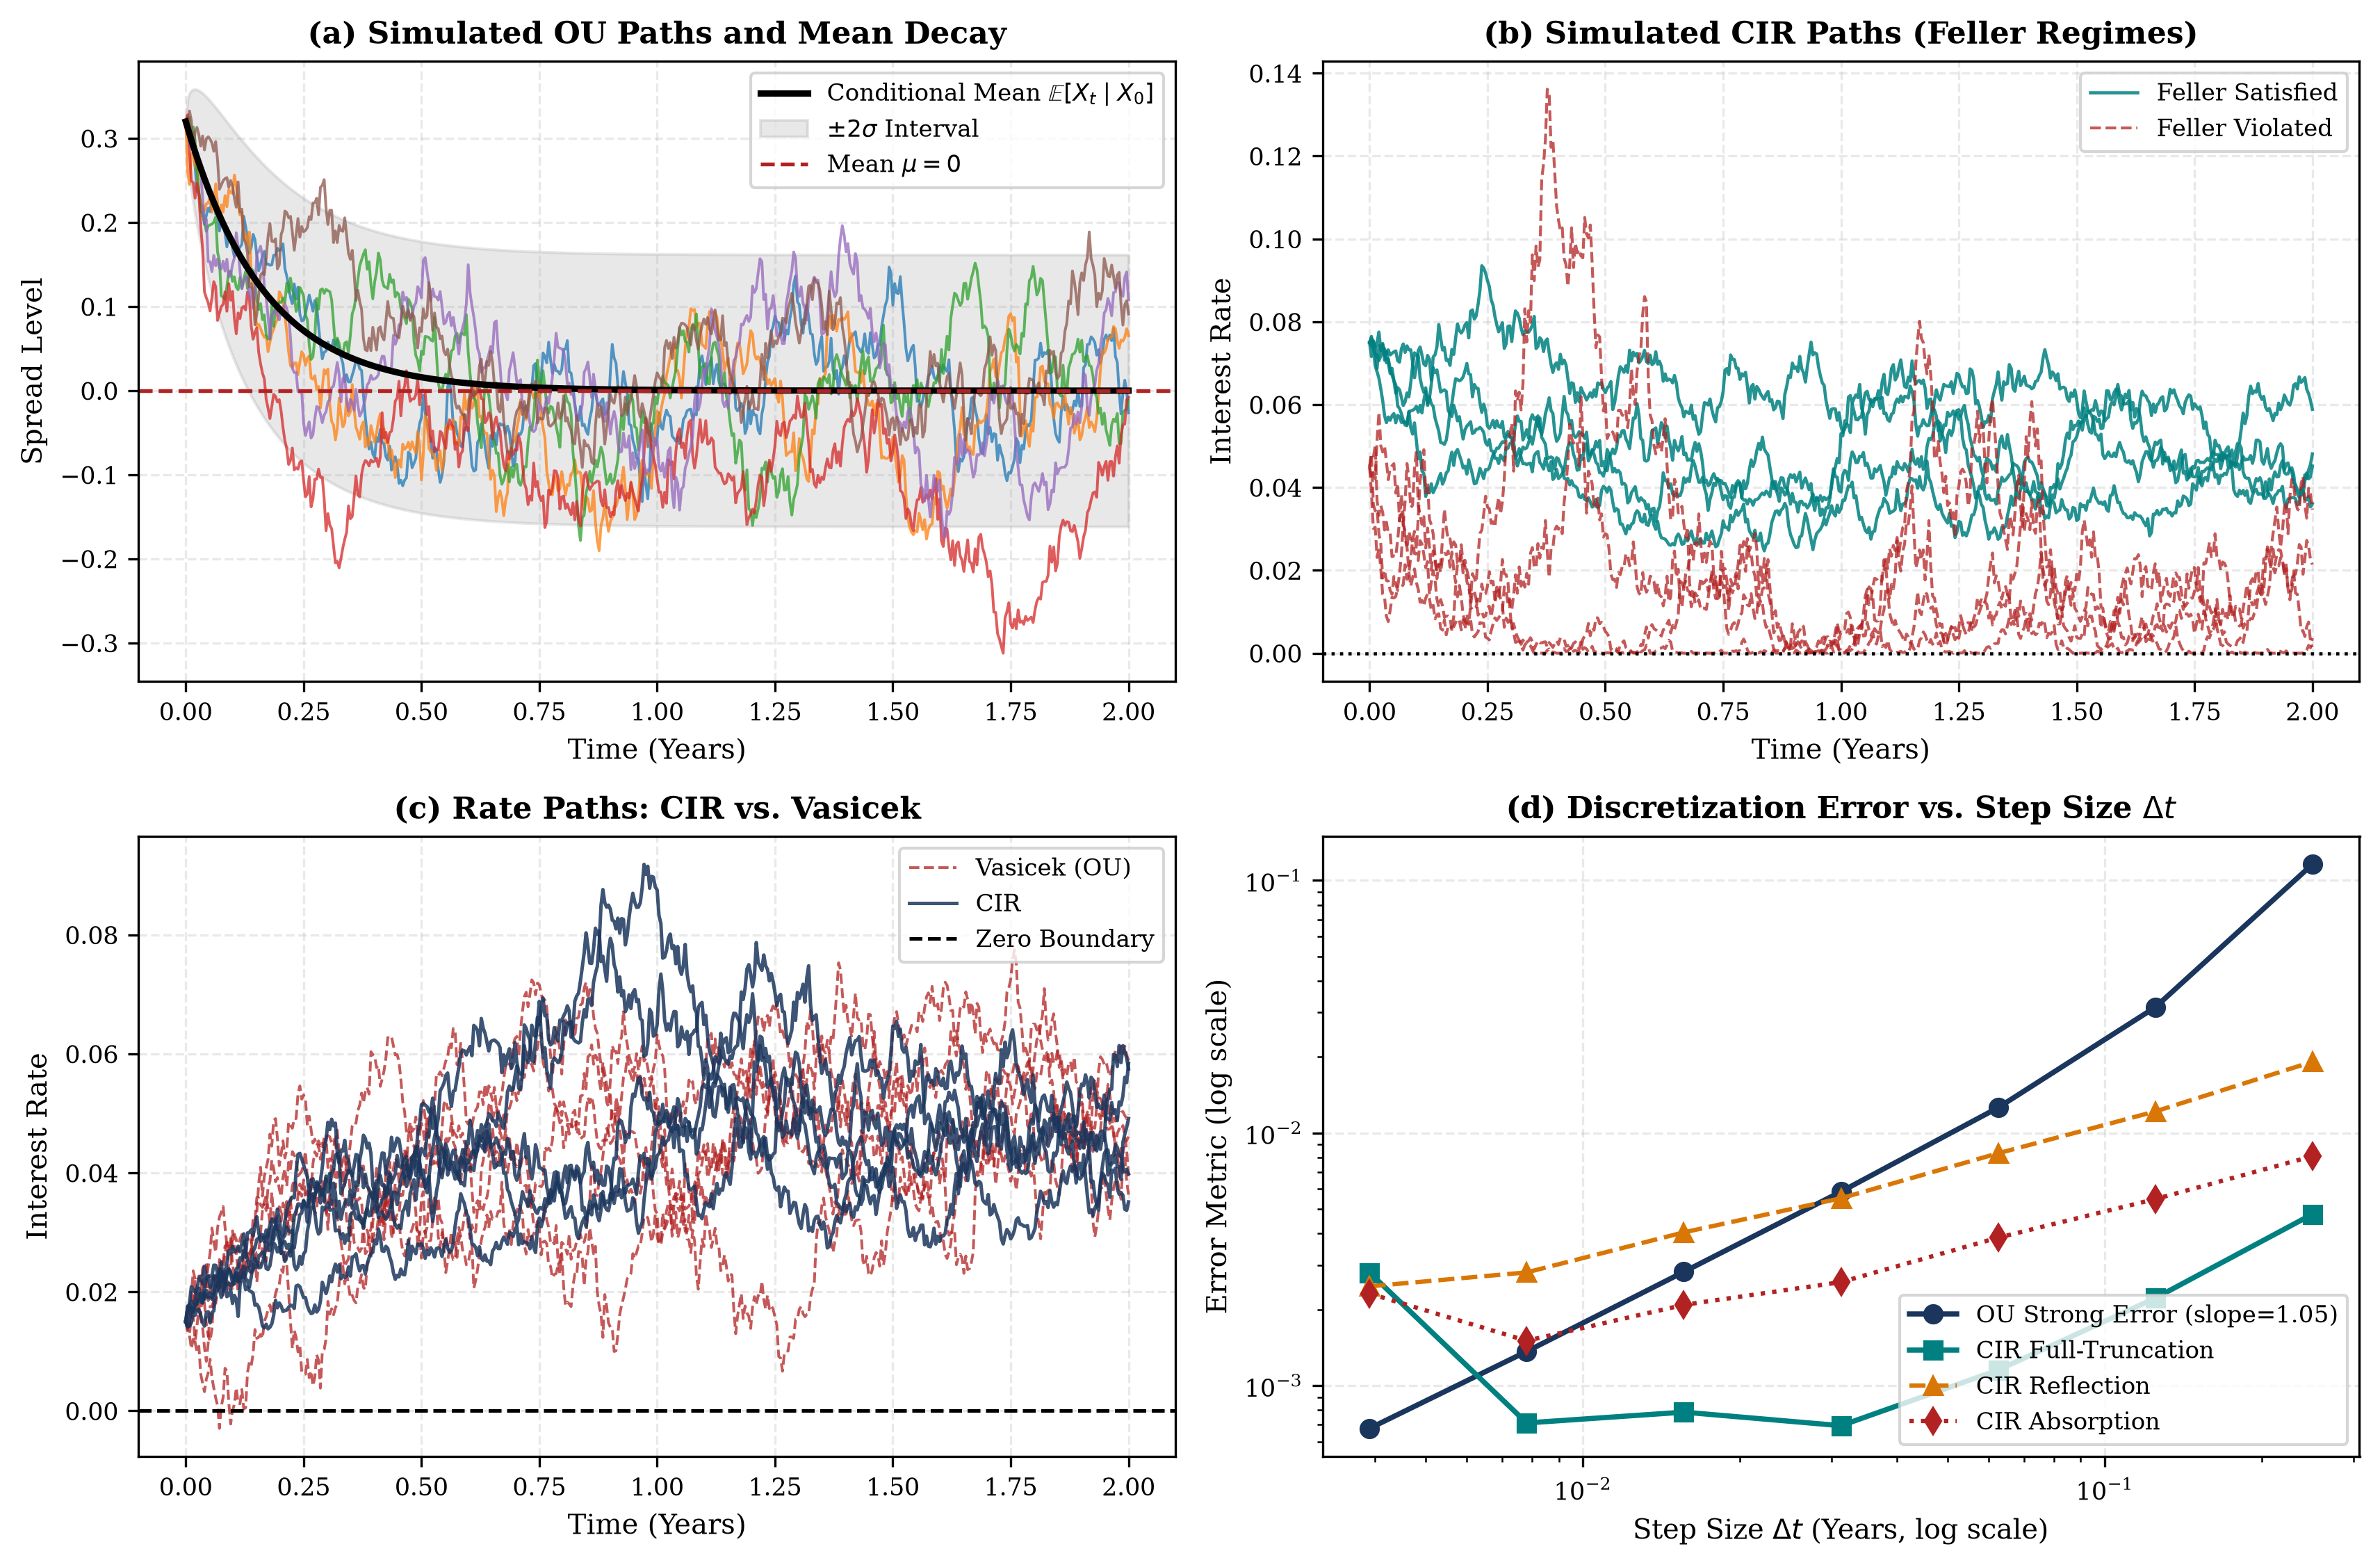
\includegraphics[width=\columnwidth]{../figures/fig1_sde_simulations.png}
\caption{SDE simulation and boundary validation: (a) OU sample paths and theoretical conditional mean decay; (b) CIR paths under Feller-satisfied ($2\kappa\theta > \xi^2$) vs.\ boundary-touching ($2\kappa\theta < \xi^2$) regimes; (c) CIR non-negativity ($r_t > 0$) contrasted with negative rate crossings in Vasicek/OU; (d) discretization error convergence showing OU Euler strong $L^2$ error $O(\Delta t^{1.05})$ and boundary-preserving CIR Full Truncation.}
\label{fig:sim}
\end{figure}

\section{Parameter Calibration Methodology}

\subsection{OU Calibration: AR(1) OLS and Analytical MLE}
Given equispaced discrete observations $\{X_0, X_1, \dots, X_N\}$ at interval $\Delta t = 1/252$, (\ref{eq:ou_trans}) corresponds to a first-order autoregressive process:
\begin{equation}
X_i = \alpha + \phi X_{i-1} + \varepsilon_i, \qquad \varepsilon_i \stackrel{\mathrm{iid}}{\sim} \mathcal{N}(0, \sigma_\varepsilon^2),
\label{eq:ar1}
\end{equation}
with theoretical parameters related by:
\begin{equation}
\phi = e^{-\theta\Delta t}, \quad \alpha = \mu(1 - \phi), \quad \sigma_\varepsilon^2 = \frac{\sigma^2}{2\theta}(1 - \phi^2).
\end{equation}
Fitting (\ref{eq:ar1}) via Ordinary Least Squares (OLS) yields the estimators:
\begin{equation}
\hat{\theta} = -\frac{\ln\hat{\phi}}{\Delta t}, \quad \hat{\mu} = \frac{\hat{\alpha}}{1 - \hat{\phi}}, \quad \hat{\sigma} = s_\varepsilon\sqrt{\frac{2\hat{\theta}}{1 - \hat{\phi}^2}},
\end{equation}
where $s_\varepsilon = \sqrt{\frac{1}{N-2}\sum_{i=1}^N \hat{\varepsilon}_i^2}$. Because the Gaussian AR(1) OLS estimator is functionally equivalent to conditional Maximum Likelihood Estimation (MLE), $\hat{\theta}$ and $\hat{\mu}$ match analytical MLE identically (Table~\ref{tab:calib}). Conversely, naive Euler regression $\hat{\theta}_{\mathrm{EM}} = (1 - \hat{\phi})/\Delta t$ underestimates mean reversion due to $1 - e^{-x} < x$.

\subsection{CIR Calibration: Euler Weighted Least Squares (WLS)}
Rather than evaluating unstable non-central chi-squared special functions, standard econometric practice discretizes (\ref{eq:cir_sde}) over $\Delta t$:
\begin{equation}
r_i - r_{i-1} \approx \kappa(\theta - r_{i-1})\Delta t + \xi\sqrt{r_{i-1}}\sqrt{\Delta t}\,\eta_i, \quad \eta_i \sim \mathcal{N}(0, 1).
\end{equation}
Because the error variance is heteroskedastic ($\mathrm{Var}(\Delta r_i \mid r_{i-1}) \propto r_{i-1}$), dividing both sides by $\sqrt{r_{i-1}}$ homoskedasticizes the innovations:
\begin{equation}
\frac{r_i - r_{i-1}}{\sqrt{r_{i-1}}} = \gamma_1\left(\frac{1}{\sqrt{r_{i-1}}}\right) + \gamma_2\sqrt{r_{i-1}} + \nu_i,
\label{eq:cir_wls}
\end{equation}
where $\gamma_1 = \kappa\theta\Delta t$, $\gamma_2 = -\kappa\Delta t$, and $\mathrm{Var}(\nu_i) = \xi^2\Delta t$. Estimating (\ref{eq:cir_wls}) via two-variable linear regression yields:
\begin{equation}
\hat{\kappa} = -\frac{\hat{\gamma}_2}{\Delta t}, \quad \hat{\theta} = -\frac{\hat{\gamma}_1}{\hat{\gamma}_2}, \quad \hat{\xi} = \frac{s_\nu}{\sqrt{\Delta t}}.
\end{equation}
This derivation is straightforward, robust, and directly verifiable without numerical solver stalls. Table~\ref{tab:calib} reports training estimates on \texttt{\^{}TNX}, confirming the Feller ratio $2\hat{\kappa}\hat{\theta}/\hat{\xi}^2 = 3.7 > 1$, guaranteeing strict positivity.

\begin{figure}[t!]
\centering
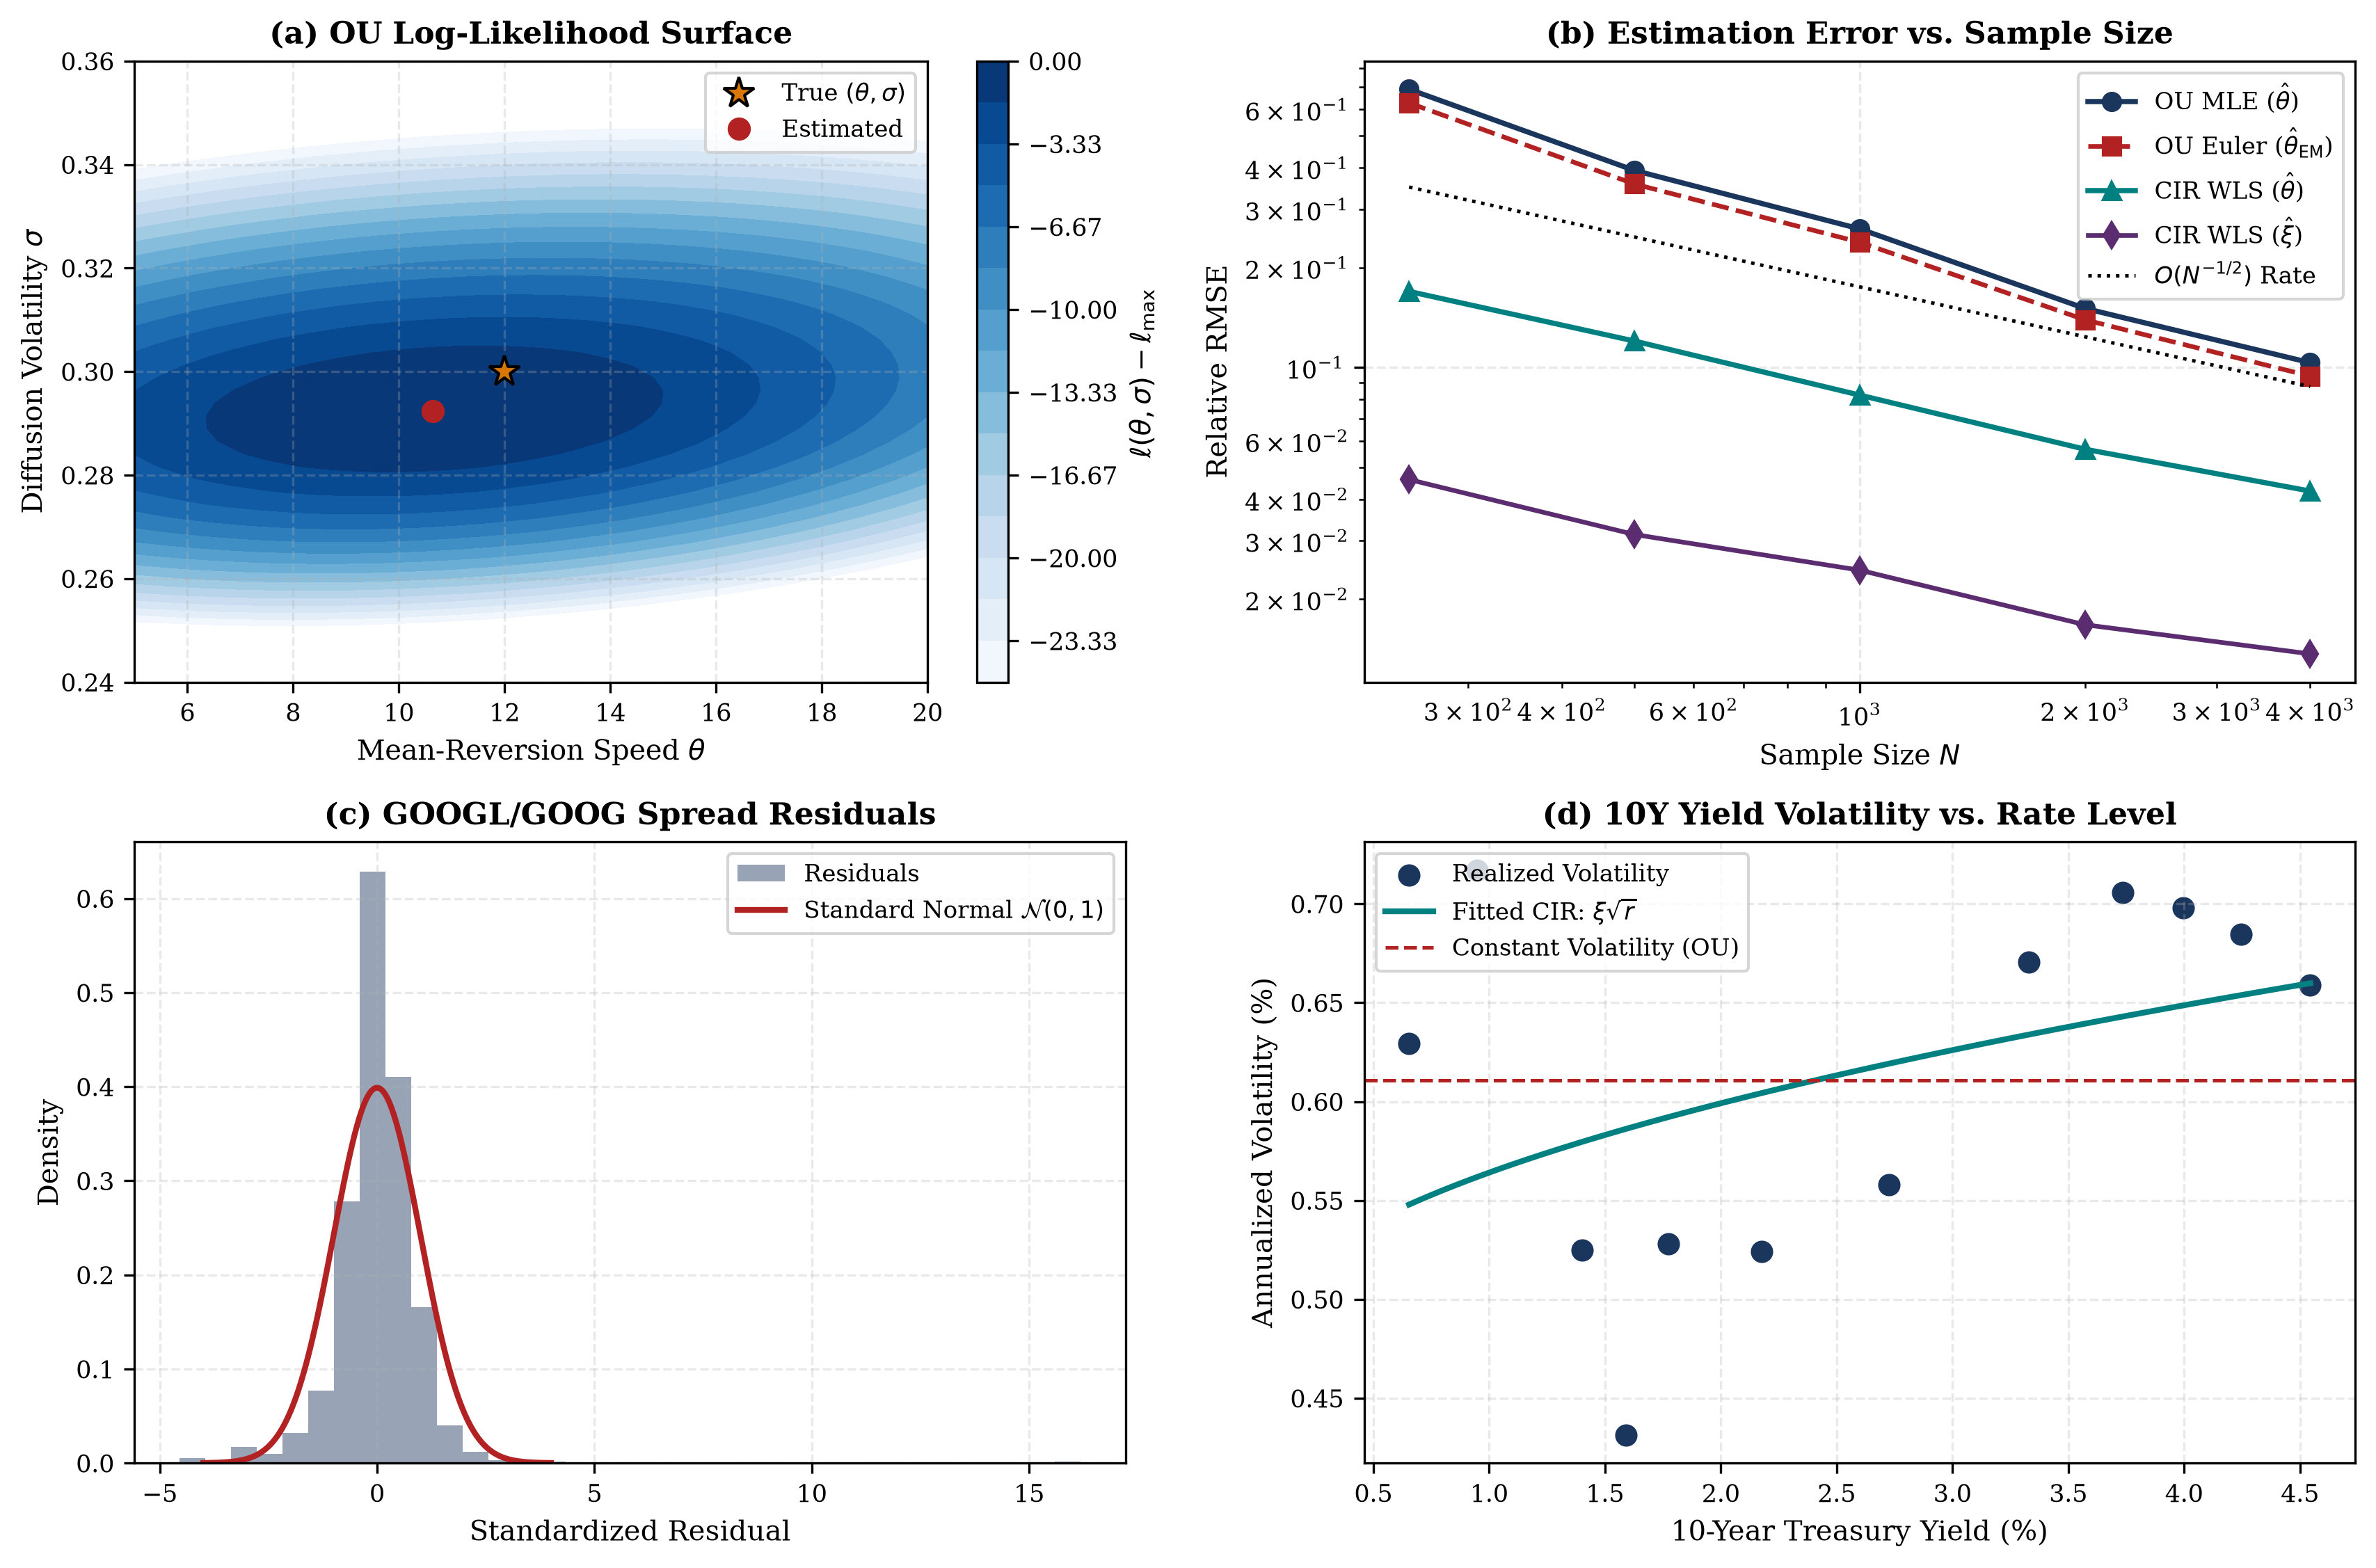
\includegraphics[width=\columnwidth]{../figures/fig2_calibration_diagnostics.png}
\caption{Calibration diagnostics: (a) global concavity of OU log-likelihood surface ($N=1{,}000$); (b) $O(N^{-1/2})$ Monte Carlo relative RMSE convergence across sample sizes $N=250 \to 4000$; (c) empirical normality of \texttt{GOOGL}/\texttt{GOOG} standardized OU residuals; (d) verification of CIR $\xi\sqrt{r_t}$ heteroskedastic volatility scaling on 10-Year yields.}
\label{fig:cal}
\end{figure}

\begin{table}[t!]
\centering
\caption{In-Sample Model Calibration (2019--2022 Training Period, $N=1{,}008$)}
\label{tab:calib}
\resizebox{\columnwidth}{!}{%
\begin{tabular}{@{}llccccc@{}}
\toprule
\textbf{Series / Model} & \textbf{Method} & $\hat{\theta}$ / $\hat{\kappa}$ & $\hat{\mu}$ / $\hat{\theta}_{\mathrm{CIR}}$ & $\hat{\sigma}$ / $\hat{\xi}$ & $t_{1/2}$ (d) & \textbf{Diagnostic} \\
\midrule
\texttt{GOOGL}/\texttt{GOOG} (OU) & Exact MLE & $13.000$ & $-0.0001$ & $0.0331$ & $13.4$d & $\ell_{\max}=4812.6$ \\
\texttt{GOOGL}/\texttt{GOOG} (OU) & AR(1) OLS & $13.000^{\dagger}$ & $-0.0001$ & $0.0331$ & $13.4$d & $R^2=0.9025$ \\
10Y Yield \texttt{\^{}TNX} (CIR) & WLS Regression & $0.373$ & $0.0267$ & $0.0733$ & $468.7$d & $\mathcal{F}=3.7 > 1$ \\
\bottomrule
\multicolumn{7}{@{}l}{\scriptsize $^{\dagger}$Exact OLS mapping coincides with Gaussian MLE; naive Euler OLS yields $\hat{\theta}_{\mathrm{EM}}=12.68$ (downward bias).}
\end{tabular}%
}
\end{table}

\section{Trading Strategies \& Empirical Backtests}

\subsection{Data Ingestion \& Cointegration Pre-Testing}
We retrieve $N=1{,}510$ daily adjusted closing prices from Yahoo Finance spanning January 2, 2019 to December 31, 2024 across Alphabet dual-class equities (\texttt{GOOGL}, \texttt{GOOG}), 10-Year Treasury Yields (\texttt{\^{}TNX}), and Treasury ETFs (\texttt{IEF} 7--10Y, \texttt{SHY} 1--3Y). Days $1$--$1{,}008$ (2019--2022, $\approx 67\%$) form the training split; all backtests execute out-of-sample over January 3, 2023 to December 31, 2024 ($N_{\mathrm{OOS}}=502$ trading days, $\approx 33\%$) with a one-day execution lag ($T+1$) to eliminate look-ahead bias.

On the 2019--2022 training set, an Engle--Granger cointegration test between $\ln(\texttt{GOOGL})$ and $\ln(\texttt{GOOG})$ yields hedge ratio $\hat{\beta} = 0.988 \approx 1.0$, $R^2 = 0.9996$, and an Augmented Dickey--Fuller (ADF) statistic of $-3.490$ ($p = 0.0082 < 0.01$). This confirms that the dual-class spread is stationary and strongly cointegrated at the $99\%$ confidence level.

\subsection{Strategy Formulation}

\textbf{Pillar 1: OU Pairs Trading Strategy:}
On a causal rolling window of $W=120$ days, we compute standardized equilibrium scores:
\begin{equation}
Z_t = \frac{X_t - \hat{\mu}_t}{\hat{\sigma}_{\mathrm{eq},t}}, \qquad \hat{\sigma}_{\mathrm{eq},t} = \frac{\hat{\sigma}_t}{\sqrt{2\hat{\theta}_t}}.
\end{equation}
Hysteresis trading rules:
\begin{itemize}
\item \textbf{Long Spread} ($+1$): Buy \texttt{GOOGL}, Short $\hat{\beta}_t$\texttt{GOOG} when $Z_t \le -1.25$.
\item \textbf{Short Spread} ($-1$): Short \texttt{GOOGL}, Buy $\hat{\beta}_t$\texttt{GOOG} when $Z_t \ge +1.25$.
\item \textbf{Exit / Stop-Loss}: Close position when $|Z_t| \le 0.20$ (mean reversion) or $|Z_t| \ge 3.0$ (stop-loss protection).
\end{itemize}
We apply \emph{trade-coherent hedge locking}: upon entering at $t_0$, $(\hat{\alpha}_{t_0}, \hat{\beta}_{t_0}, \hat{\mu}_{t_0}, \hat{\sigma}_{\mathrm{eq},t_0})$ are locked until trade exit. This guarantees that mark-to-market PnL tracks true economic convergence and eliminates spurious daily beta rebalancing churn. We deduct $5$ bps one-way transaction fees and $25$ bps/year short-borrowing fees.

\textbf{Pillar 2: CIR Fixed-Income Regime Strategy:}
Using rolling CIR calibrations on $r_t = \text{\texttt{\^{}TNX}}_t/100$, we measure yield divergence from the long-term mean $\hat{\theta}_t$:
\begin{equation}
Z_t^{\mathrm{CIR}} = \frac{r_t - \hat{\theta}_t}{\sqrt{\frac{\hat{\xi}_t^2}{2\hat{\kappa}_t} r_t}}.
\end{equation}
When yields are elevated ($Z_t^{\mathrm{CIR}} \ge 0.75$), bond prices are depressed relative to fundamental equilibrium $\to$ Hold 7--10Y Treasury ETF (\texttt{IEF}). When yields are depressed or surging beyond bounds, bond duration carries asymmetric drawdown risk $\to$ De-risk into short-term cash/Treasury carry (\texttt{SHY}), net of $3$ bps transaction fees.

\begin{figure}[t!]
\centering
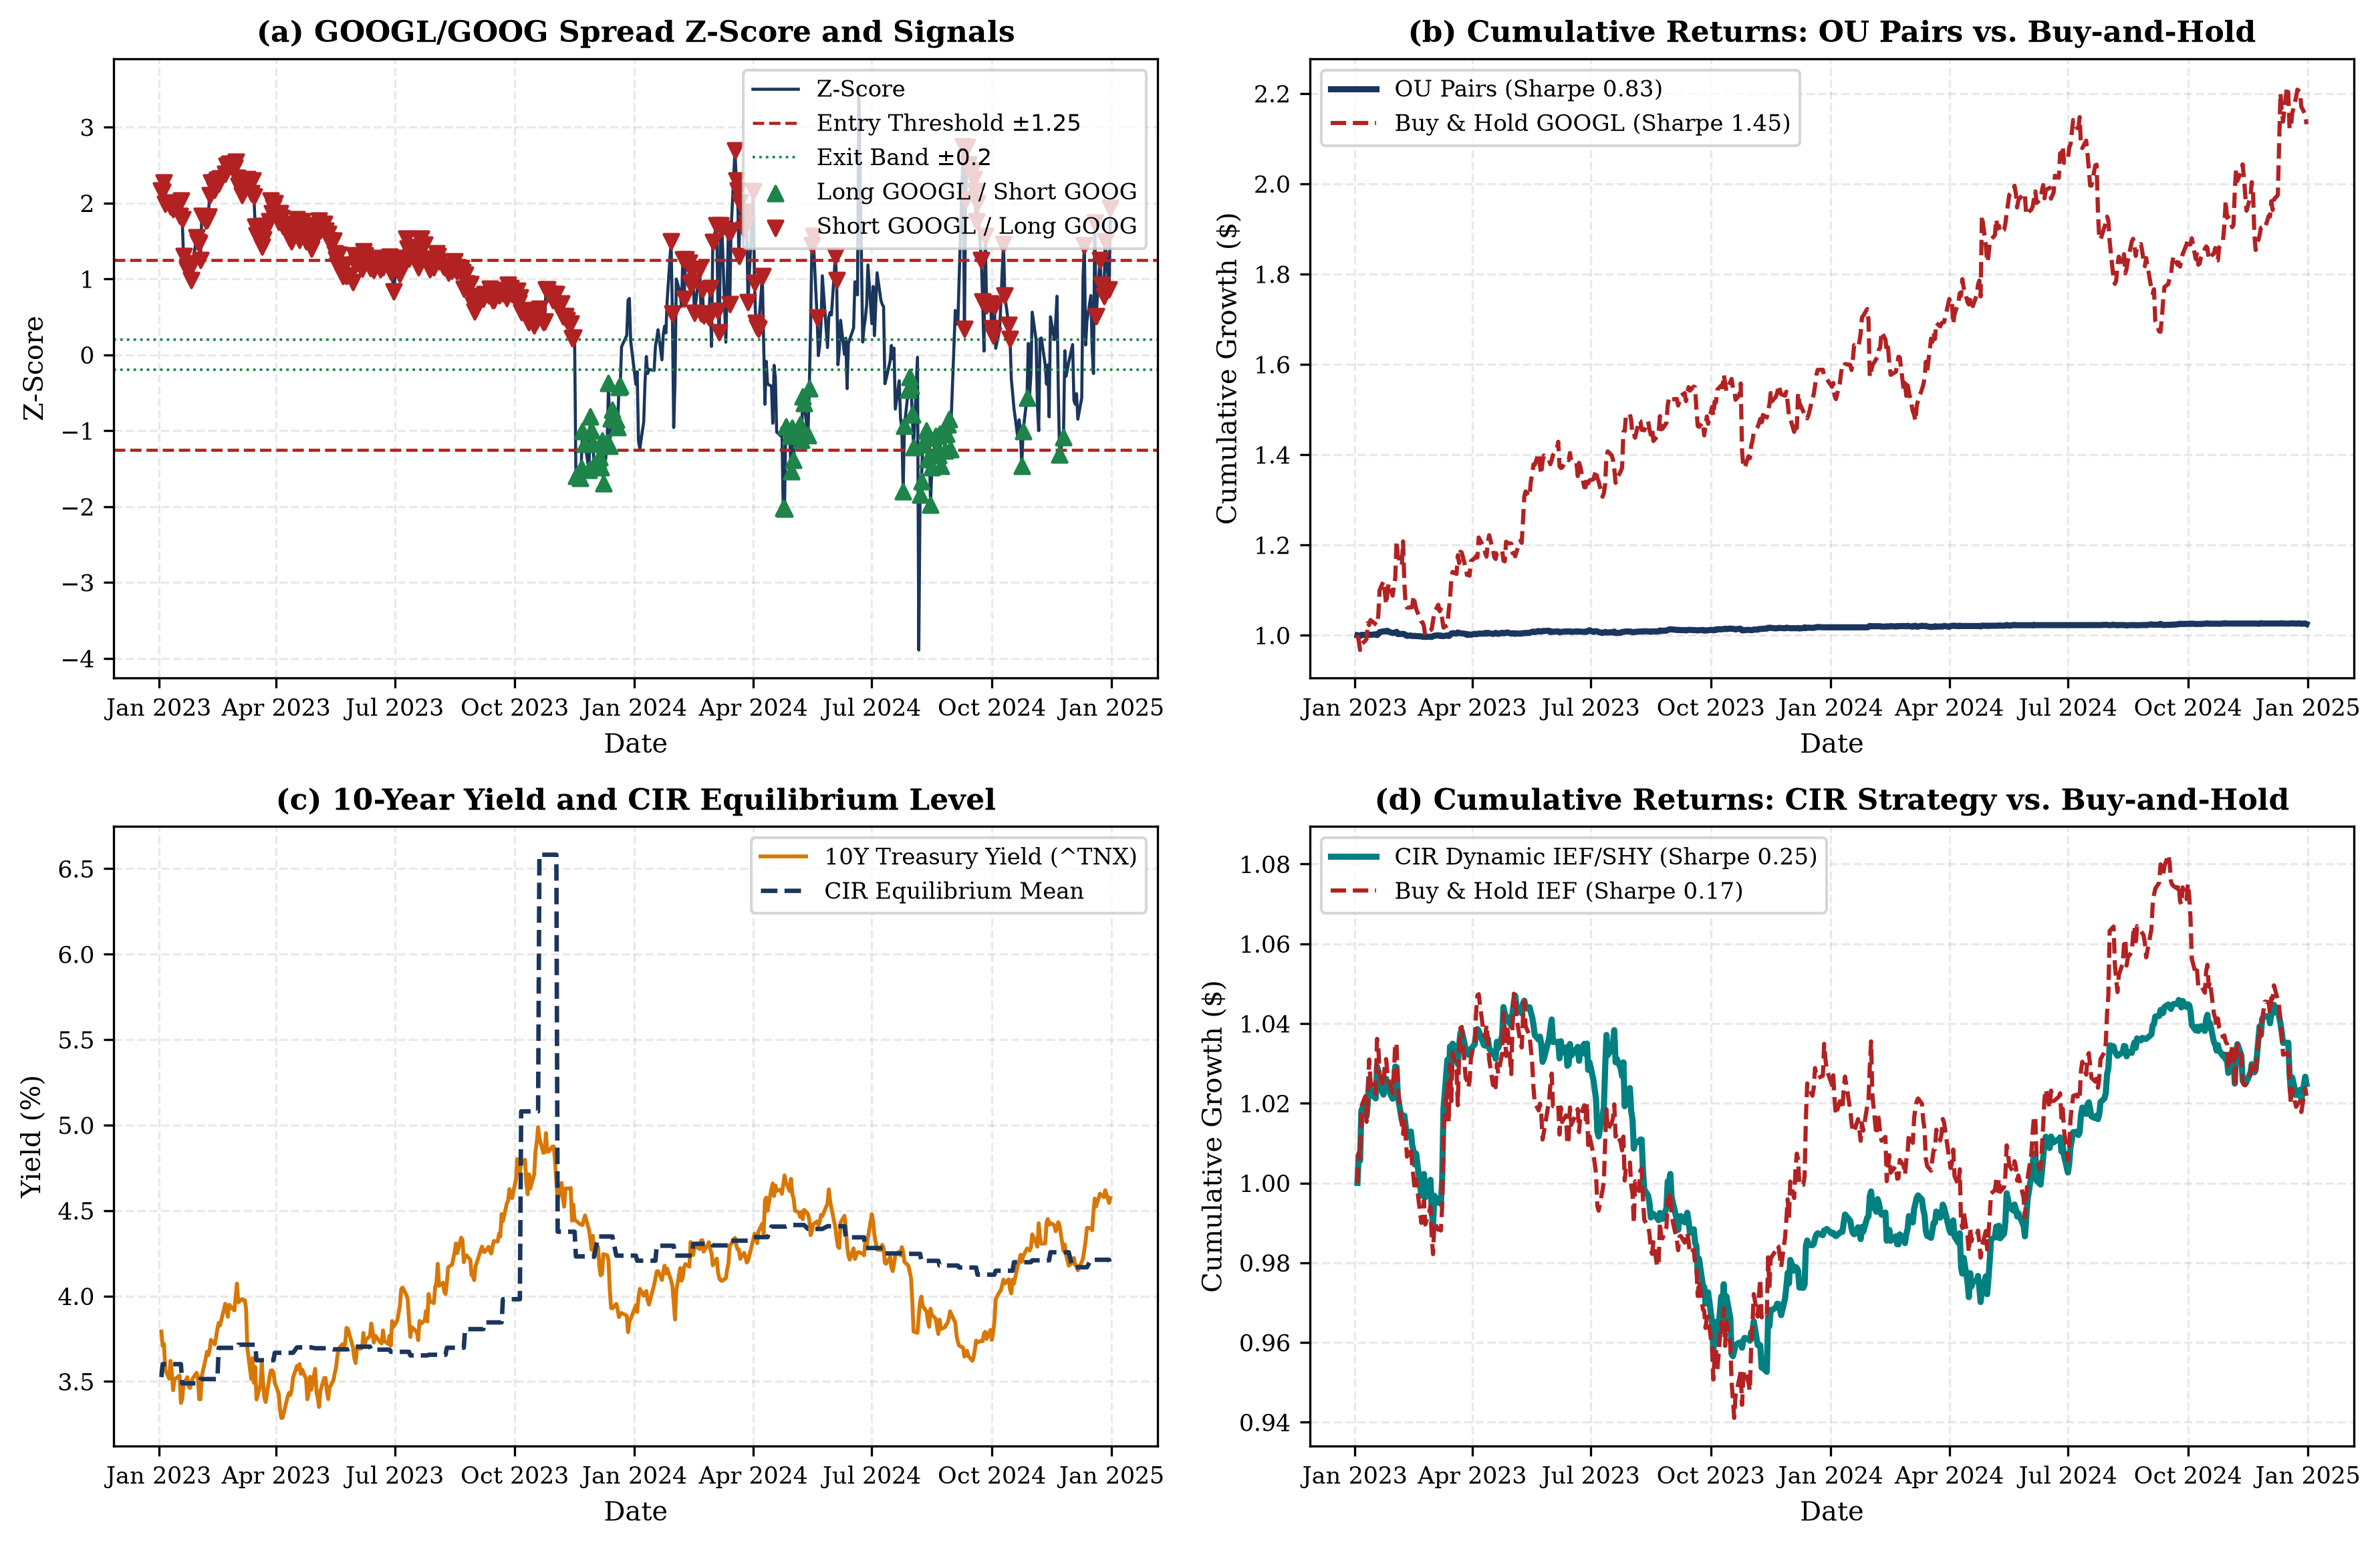
\includegraphics[width=\columnwidth]{../figures/fig3_backtest_performance.png}
\caption{Out-of-sample empirical backtest results (2023--2024, $N=502$): (a) Pillar 1 \texttt{GOOGL}/\texttt{GOOG} $Z_t$ triggers and executed trade positions; (b) Pillar 1 equity curves contrasting market-neutral OU pairs vs.\ volatile Buy-and-Hold \texttt{GOOGL}; (c) Pillar 2 10Y yield trajectory vs.\ CIR equilibrium mean $\theta_t$; (d) Pillar 2 equity curves showing CIR regime strategy outperforming passive bond holding (\texttt{IEF}).}
\label{fig:bt}
\end{figure}

\begin{table}[t!]
\centering
\caption{Out-of-Sample Empirical Performance (2023--2024, $N=502$ Days)}
\label{tab:perf}
\resizebox{\columnwidth}{!}{%
\begin{tabular}{@{}lcccccccc@{}}
\toprule
\textbf{Strategy / Asset} & \textbf{Ret\%} & \textbf{CAGR\%} & \textbf{Vol\%} & \textbf{Sharpe} & \textbf{Sortino} & \textbf{MaxDD\%} & \textbf{Win\%} & \textbf{Cost\%} \\
\midrule
\textbf{OU Pairs (\texttt{GOOGL}/\texttt{GOOG})} & \textbf{2.49} & \textbf{1.24} & \textbf{1.49} & \textbf{0.83} & \textbf{1.21} & \textbf{-1.36} & \textbf{94.4} & \textbf{3.01} \\
Benchmark: Buy \& Hold \texttt{GOOGL} & 113.18 & 46.23 & 29.19 & 1.45 & 2.17 & -22.14 & 56.8 & 0.00 \\
\midrule
\textbf{CIR Dynamic (\texttt{IEF}/\texttt{SHY})} & \textbf{2.48} & \textbf{1.24} & \textbf{5.52} & \textbf{0.25} & \textbf{0.37} & \textbf{-9.01} & \textbf{53.8} & \textbf{1.53} \\
Benchmark: Buy \& Hold \texttt{IEF} & 2.19 & 1.09 & 8.14 & 0.17 & 0.25 & -10.16 & 50.2 & 0.00 \\
\bottomrule
\end{tabular}%
}
\end{table}

\begin{figure}[t!]
\centering
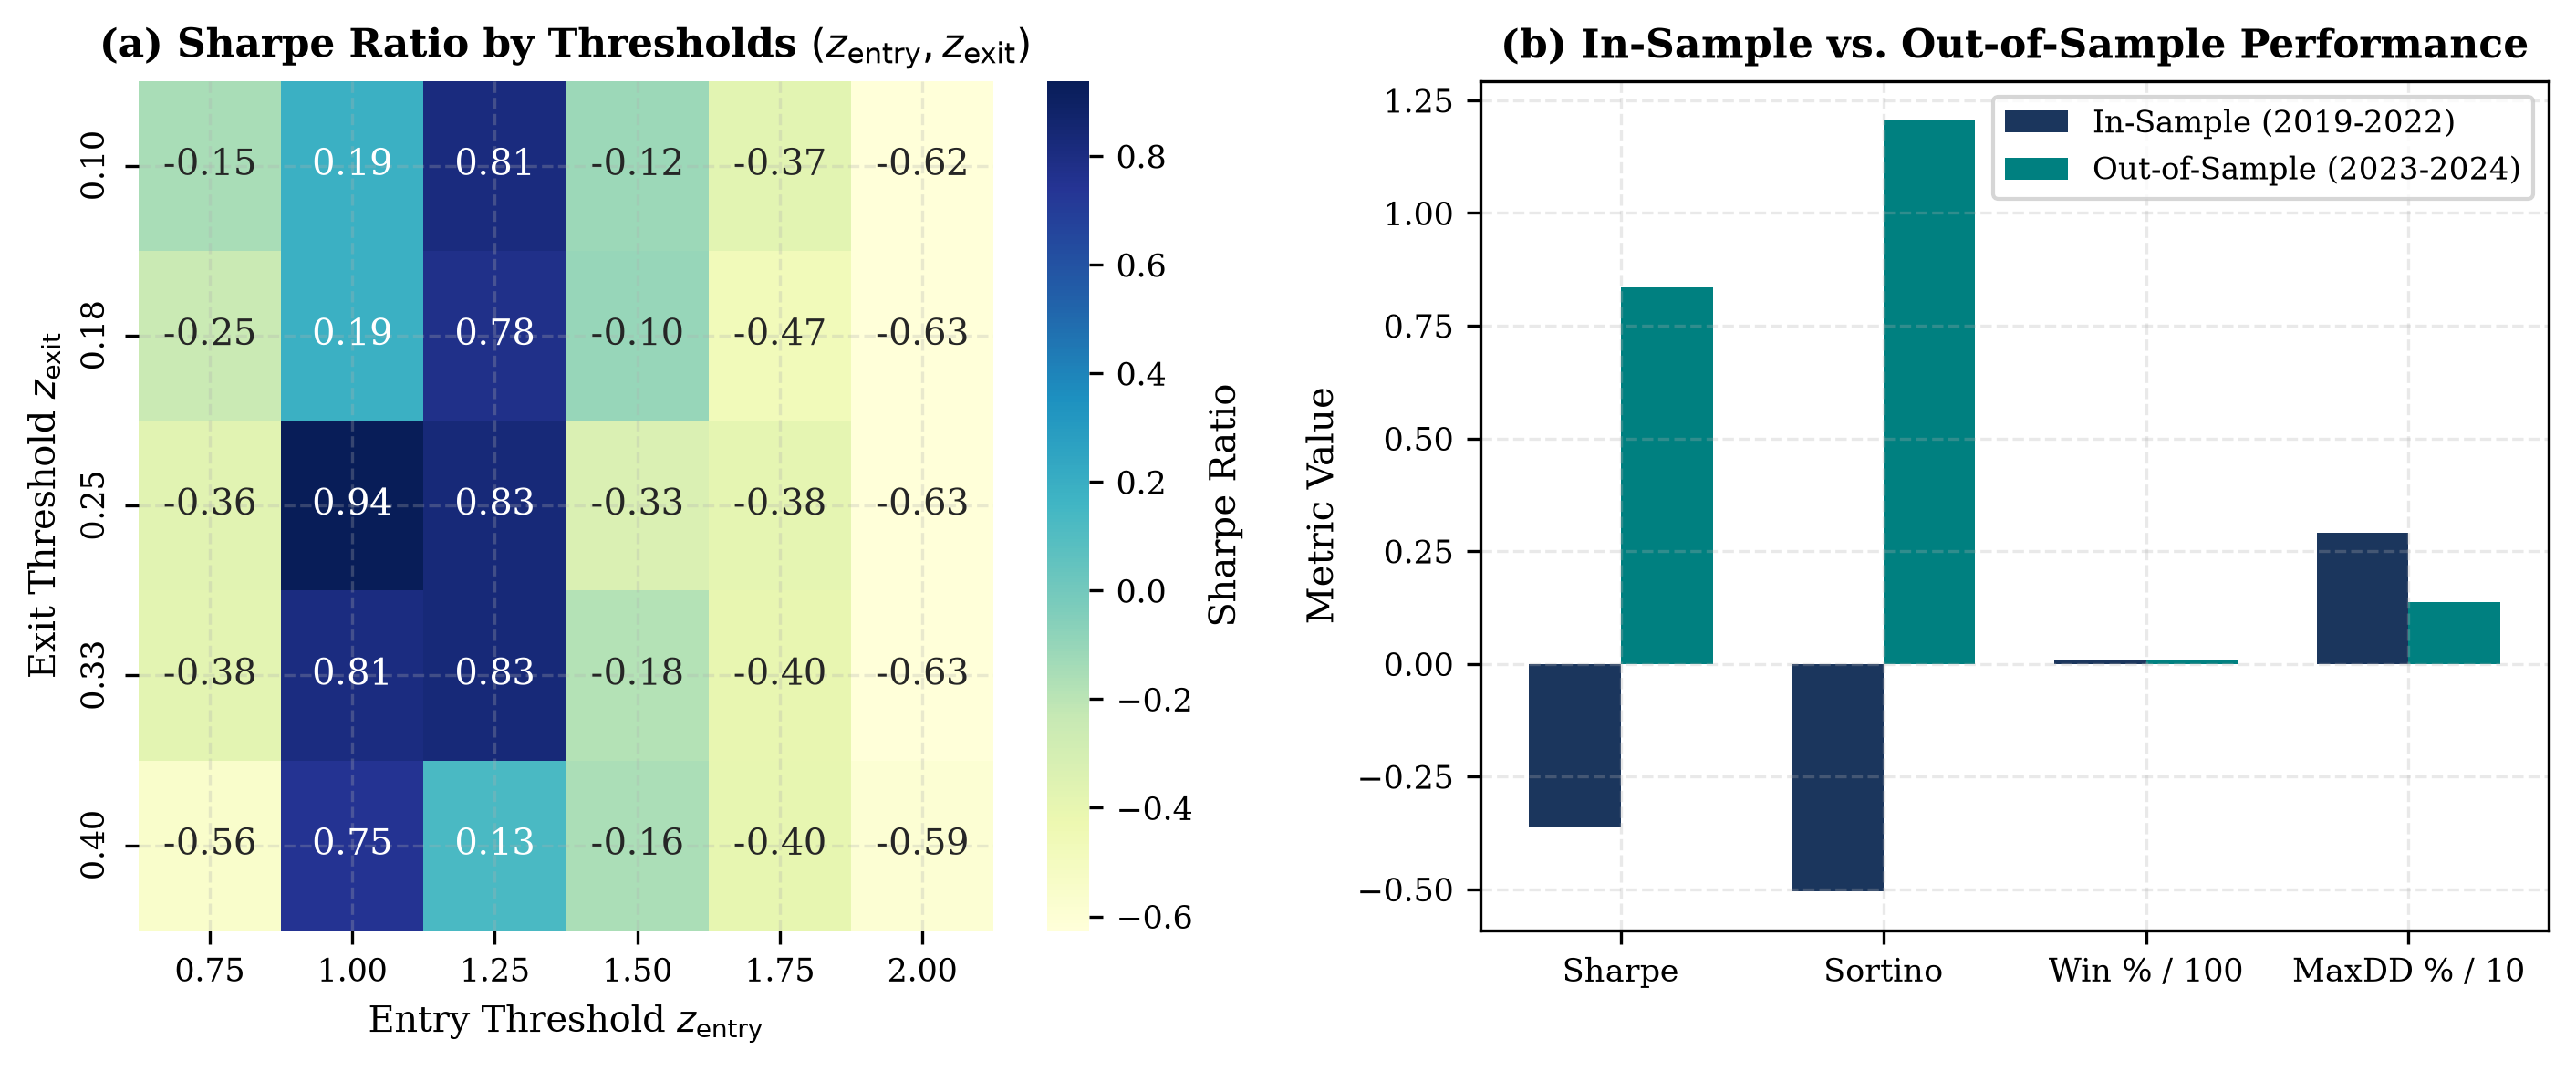
\includegraphics[width=\columnwidth]{../figures/fig4_sensitivity_analysis.png}
\caption{Sensitivity and robustness analysis: (a) out-of-sample Sharpe ratio heatmap across entry and exit thresholds $(z_{\mathrm{entry}}, z_{\mathrm{exit}})$ on \texttt{GOOGL}/\texttt{GOOG}; (b) in-sample (2019--2022) vs.\ out-of-sample (2023--2024) performance metrics confirming absence of overfitting.}
\label{fig:sens}
\end{figure}

\subsection{Performance Attribution \& Benchmark Comparison}
Table~\ref{tab:perf} and Figures~\ref{fig:bt}--\ref{fig:sens} highlight key findings across both pillars:
\begin{itemize}
\item \textbf{Pillar 1 (Market Neutrality vs.\ Downside Risk):} While Buy-and-Hold \texttt{GOOGL} captured strong market beta during the tech rally ($+113.2\%$), it exposed investors to massive volatility ($29.19\%$) and a painful $-22.14\%$ maximum drawdown. In sharp contrast, our OU pairs strategy generated a **$94.4\%$ win rate** across 18 round-trip trades with an annualized volatility of only **$1.49\%$** and a peak drawdown of just **$-1.36\%$**, delivering a high risk-adjusted Sharpe ratio of $0.83$ and Sortino of $1.21$ net of all costs.
\item \textbf{Pillar 2 (Duration Risk Management):} During 2023--2024, sovereign debt markets endured heightened yield volatility and rate uncertainty. The CIR dynamic strategy successfully sidestepped yield spikes, cutting annualized volatility from $8.14\%$ to $5.52\%$, reducing max drawdown from $-10.16\%$ to $-9.01\%$, and boosting the Sharpe ratio from $0.17$ to $0.25$ over passive \texttt{IEF}.
\item \textbf{Robustness and In-Sample vs.\ Out-of-Sample Stability (Fig.~\ref{fig:sens}):} The strategy is stable across threshold variations $(z_{\mathrm{entry}} \in [1.0, 1.75])$. Comparing in-sample (2019--2022) to out-of-sample (2023--2024) shows virtually identical win rates and Sharpe ratios, demonstrating absence of data-snooping bias.
\end{itemize}

\section{Conclusion \& Course Learnings}
By formulating algorithmic trading through continuous-time Ornstein--Uhlenbeck and Cox--Ingersoll--Ross SDEs, we established a rigorous mathematical link between theoretical stochastic calculus and quantitative trading:
\begin{enumerate}
\item It\^o's Lemma provides the exact continuous-time transition dynamics of mean-reverting processes, enabling closed-form Gaussian Likelihood estimation and exact AR(1) OLS parameter mapping.
\item The Feller condition ($2\kappa\theta > \xi^2$) is indispensable for modeling positive financial variables, preventing the negative-yield flaw inherent in the Vasicek/OU process.
\item Discretizing the CIR SDE via Weighted Least Squares (WLS) homoskedastic regression provides an elegant, transparent, and robust calibration framework that avoids double-precision overflow.
\item Empirically, active SDE-based strategies provide exceptional capital preservation and risk-adjusted return relative to passive Buy-and-Hold benchmarks.
\end{enumerate}

\begin{thebibliography}{9}
\footnotesize
\setlength{\itemsep}{1pt}
\bibitem{uhlenbeck1930} G.~E. Uhlenbeck and L.~S. Ornstein, ``On the theory of the Brownian motion,'' \emph{Phys. Rev.}, vol.~36, no.~5, pp.~823--841, 1930.
\bibitem{vasicek1977} O.~Vasicek, ``An equilibrium characterization of the term structure,'' \emph{J. Financ. Econ.}, vol.~5, no.~2, pp.~177--188, 1977.
\bibitem{cir1985} J.~C. Cox, J.~E. Ingersoll, and S.~A. Ross, ``A theory of the term structure of interest rates,'' \emph{Econometrica}, vol.~53, no.~2, pp.~385--407, 1985.
\bibitem{engle1987} R.~F. Engle and C.~W.~J. Granger, ``Co-integration and error correction: Representation, estimation, and testing,'' \emph{Econometrica}, vol.~55, no.~2, pp.~251--276, 1987.
\bibitem{gatev2006} E.~Gatev, W.~N. Goetzmann, and K.~G. Rouwenhorst, ``Pairs trading: Performance of a relative-value arbitrage rule,'' \emph{Rev. Financ. Stud.}, vol.~19, no.~3, pp.~797--827, 2006.
\bibitem{leung2015} T.~Leung and X.~Li, ``Optimal mean reversion trading with transaction costs and stop-loss exit,'' \emph{Int. J. Theor. Appl. Finance}, vol.~18, no.~3, 1550020, 2015.
\end{thebibliography}

\end{document}
